\documentclass[11pt,letterpaper,final]{report}
\usepackage[utf8]{inputenc}
\usepackage[english]{babel}
\usepackage{amsmath}
\usepackage{indentfirst}
\usepackage{amsfonts}
\addto{\captionsenglish}{\renewcommand{\bibname}{\LARGE{References}}}
\usepackage{pdfpages}
\usepackage{subcaption}
\usepackage{etoolbox}
\usepackage{amssymb}
\usepackage[font=small,labelfont=bf]{caption}
\usepackage{hanging}
\usepackage{notoccite}
\usepackage{float}
\usepackage{makeidx}
\usepackage{color}
\usepackage{titlesec}
\usepackage{gensymb}
\usepackage{hyperref}
\usepackage{graphicx}
\usepackage{lmodern}

\makeatletter
% section from book
%\newcommand\section{\@startsection {section}{1}{\z@}%
%                                   {-3.5ex \@plus -1ex \@minus -.2ex}%
%                                   {2.3ex \@plus.2ex}%
%                                   {\normalfont\Large\bfseries}}
\renewcommand\chapter{\@startsection {chapter}{0}{\z@}%
                                   {-4.5ex \@plus -1ex \@minus -.2ex}%
                                   {3.3ex \@plus.2ex}% 
                                   {\normalfont\LARGE\textbf}}


\makeatletter



\setlength{\parskip}{\baselineskip}%
\setlength{\parindent}{0pt}%






\usepackage{fourier}
\usepackage[left=1in,right=1in,top=1in,bottom=1in]{geometry}

\titleformat{\chapter}{\normalfont\huge}{\thechapter.}{20pt}{\huge\bf}
\titlespacing*{\chapter}{0pt}{-.5in}{20pt}
\author{Charles Hammond \\ Jaime Luo \\ Jacob Newman}


\begin{document}



\begin{center}

\begin{huge} 

\begin{Huge}\textbf{Work Plan} \end{Huge} \\~\\  UV System Replacement/UVT Requirement Reduction \\~\\
\end{huge}


\begin{Large} \textit{pHlux Engineering} \end{Large}



\begin{large}

\vspace{100pt}

\includegraphics[height=1.5in]{wp1}\\
\end{large}

\vspace{100pt}


\begin{tabular}{ll}
    \textbf{Prepared by:}&Charles Hammond\\
                         & Jaime Luo\\
                         & Jacob Newman\\
                         & \\~\\
    \textbf{Prepared for:}& Colleen Bronner\\
                         & \\~\\
    \textbf{Finalized on:}& \today\\ 

\end{tabular}

\end{center}

\pagenumbering{gobble}


\newpage
\setcounter{page}{0}


%%%%%%%%%%%%%%%%%%%%%%%%%%%%%%%%%%%%%%%%%%%%%%%%%%%%%%%%%%%%%
%%%%%%%%%%%%%%%%%%%%% Executive Summary %%%%%%%%%%%%%%%%%%%%%
%%%%%%%%%%%%%%%%%%%%%%%%%%%%%%%%%%%%%%%%%%%%%%%%%%%%%%%%%%%%%


\chapter*{Executive Summary}
\pagenumbering{roman} 

    \addcontentsline{toc}{chapter}{Executive Summary}

    This report contains the storm water management design requested by the city of Davis, California, on April 18th, 2018. The sources of stormwater are a tarmac, a grass-covered park, and a housing developement. The design includes a conveyance channel, gutters, inlets and a storm sewer for the housing development, a culvert, and a detention pond. The design is based on a 10-year storm.



    
    
\newpage
\setlength{\parskip}{0pt}%
\tableofcontents
\newpage
\listoffigures

\setlength{\parskip}{\baselineskip}%
\addcontentsline{toc}{chapter}{List of Figures}


\newpage
\chapter*{Nomenclature}
\addcontentsline{toc}{chapter}{Nomenclature}

\begin{table}[htbp]
\centering
\begin{tabular}{ccc}
\textbf{Symbol/Initialism} & \textbf{Meaning} & \textbf{Units} \\
\hline
NPDES & National Pollution Discharge Elimination System &  \\
UVT & Ultraviolet Transmissivity & \\
WWTP & Wastewater Treatment Plant & \\
CVRWQCB & Central Valley Regional Water Quality Control Board & \\
MPN & Most probable number &  \\
mgd & Million gallons per day & $10^6$ gal/day \\
ADP & Advanced Disinfection Process & \\







\end{tabular} 
\end{table}


\newpage
\setcounter{chapter}{0}
\setcounter{figure}{0}
\setcounter{section}{0}

%%%%%%%%%%%%%%%%%%%%%%%%%%%%%%%%%%%%%%%%%%%%%%%%%%%%%%%%%%%%%%%%%%%%
%%%%%%%%%%%%%%%%%%%%% 1.0 Statement of Problem %%%%%%%%%%%%%%%%%%%%%
%%%%%%%%%%%%%%%%%%%%%%%%%%%%%%%%%%%%%%%%%%%%%%%%%%%%%%%%%%%%%%%%%%%%

\chapter{Statement of Problem}
\setcounter{page}{0}
\pagenumbering{arabic}
There are two problems that this project aims to solve for the UC Davis wastewater treatment plant (WWTP). First, the minimum UVT requirement of 55\% in the NPDES permit governing the plant results in yearly violations and fines. These violations are undesirable both financially, as the fines add up year after year, and legally, because willfully violating the law is not a viable or responsible solution. To resolve this, the UCD Utilities Division has requested a letter to the Water Board that justifies, based on data and rigorous testing, the reduction or removal of the UVT limit.

Second, the UV disinfection system is nearing the end of its planned service life and is in need of replacement. Because the WWTP discharges to Putah Creek, the Arboretum, and is even used for cooling buildings, the safety and compliance of the recycled water is of the utmost importance. An aging disinfection system could lead to water quality and reliability issues, which could lead to violations, fines, and perhaps even lawsuits. Thus, a replacement design has been requested by the UCD Utilities Division.




%%%%%%%%%%%%%%%%%%%%%%%%%%%%%%%%%%%%%%%%%%%%%%%%%%%%%%%%%%%%%%%%%%
%%%%%%%%%%%%%%%%%%%%% 2.0 Project Objectives %%%%%%%%%%%%%%%%%%%%%
%%%%%%%%%%%%%%%%%%%%%%%%%%%%%%%%%%%%%%%%%%%%%%%%%%%%%%%%%%%%%%%%%%

\setcounter{figure}{0}
\setcounter{section}{0} 
\chapter{Project Objectives}

There are two major objectives for this project:
\begin{enumerate}
\item Craft a memorandum intended for the Water Board that uses data from Carollo’s bioassay testing to justify the reduction or removal of the UVT requirement in the UC Davis WWTP’s NPDES permit.

\item Design a disinfection system that satisfies Title 22, fits within the current UV disinfection system footprint, utilizes the existing infrastructure, and minimizes energy consumption and cost.

\end{enumerate}

Success in completing these objectives will be measured by evaluating feedback from the client and by comparing actual vs. planned progress as detailed in the project timeline.



%%%%%%%%%%%%%%%%%%%%%%%%%%%%%%%%%%%%%%%%%%%%%%%%%%%%%%%%%%
%%%%%%%%%%%%%%%%%%%%% 3.0 Background %%%%%%%%%%%%%%%%%%%%%
%%%%%%%%%%%%%%%%%%%%%%%%%%%%%%%%%%%%%%%%%%%%%%%%%%%%%%%%%%

\setcounter{figure}{0}
\setcounter{section}{0}
\setcounter{table}{0}
\chapter{Background}

Wastewater treatment is usually divided into three main stages: primary, secondary, and tertiary. Primary treatment involves the removal of suspended solids and organic matter, secondary treatment typically includes the biological oxidation of organics remaining in the primary effluent, and tertiary treatment employs filters and/or disinfection processes to produce recycled water \cite{Metcalf}.
				 					
Disinfection is the process of destroying or inactivating pathogenic organisms, and considering the potential for human exposure to recycled wastewater, proper disinfection is extremely important. Of particular concern are bacteria, protozoan oocysts and cysts, viruses, and helminth ova, all of which can cause serious illness \cite{Metcalf}. Although many bacteria are harmless or beneficial, some present serious human health risks; for example, \textit{Legionella pneumophila} can cause malaise, myalgia, fever, headache, and respiratory illness \cite{Metcalf}.

Wastewater is usually disinfected with either chemical agents, such as chlorine or ozone, or non-ionizing radiation, most commonly ultraviolet light (UV) \cite{Metcalf}. Chlorine and ozone mainly function by oxidizing and destroying cell walls, while UV works mainly by damaging the RNA and DNA within a cell, rendering it incapable of reproducing \cite{Metcalf}. Combined UV-chemical treatments are known as UV-based advanced disinfection processes. For example, research has suggested that combining UV treatment with H$_2$O$_2$ could enhance viral deactivation \cite{Peizhe}. Each method has its strengths and weaknesses and each WWTP should tailor its disinfection process to its particular needs. For example, using chlorine or ozone can result in toxic disinfection byproducts (DPB), and while some viruses are resistant to UV irradiation, because UV disinfection works primarily by dimerizing adjacent thymine and cytosine DNA/RNA molecules, pathogens with thymine-rich genetic material (e.g., \textit{C. parvum} and Adenovirus) are more sensitive to UV disinfection \cite{Metcalf},\cite{ELShahawy2019}.

UV light is electromagnetic radiation with wavelengths between 100-400 nm, which is divided into longwave (UV-A), middlewave (UV-B), and shortwave (UV-C). The wavelength used for for disinfection is 254 nm and is generated by striking an electric arc between two electrodes in a lamp containing mercury\cite{ELShahawy2019}. UV lamps come in three general categories, 1) low-pressure, low-intensity (LPLI), 2) low-pressure, high-intensity (LPHI), and 3) medium-pressure, high intensity (MPHI) \cite{Metcalf}. Among the three types, LPLI and LPHI lamps are the most efficient, with 30-50\% and 35-50\% of their energy output in the form of monochromatic 254 nm wavelength light, respectively. MPHI lamps produce more intense light, but much less efficiently, with only 15-20\% of their energy output in the germicidal range \cite{Metcalf}.

The effectiveness of a given UV disinfection system depends on the chemical characteristics of the wastewater, presence of particulate matter, the target organisms, and the system design \cite{Metcalf}. These factors all influence the UV “dose”, which is defined as 



\setlength{\parskip}{0pt}
\begin{equation}
    D=I_{avg} \times t
  \end{equation}
  \begin{align*}
    \text{Where }&D= dose [mJ/cm^2]\\
    & I_{avg}= \text{average UV intensity }[mW/cm^2]\\
    & t=\text{exposure time,} s
  \end{align*}

  \setlength{\parskip}{\baselineskip}

Constituents in wastewater can influence the dose by reducing the average UV intensity. Typically these effects are measured via absorbance and transmittance, which is why the National Water Resources Institute (NWRI) recommends a general minimum of 55\% UV transmissivity for a UV dose of 100 $mJ/cm^2$ \cite{NPDES}. Dissolved iron and organic compounds with double bonds and aromatic functional groups are the most influential constituents, as they can directly absorb UV light \cite{Metcalf}. Particles can reduce disinfection performance by shielding harmful organisms from irradiation, reflecting and/or refracting light, and by harboring microorganisms \cite{Metcalf}.

Contact basins can be either open channels or closed reactors and, due to the relatively short contact time, they must be carefully designed to ensure complete disinfection \cite{Metcalf}. Hydraulic design of a UV disinfection system is extremely important, as non-ideal hydraulics can lead to longitudinal mixing, which leads to a distributed, rather than uniform, exposure time \cite{Metcalf}. Two important challenges when designing a UV disinfection system are ensuring uniform velocity fields approaching and exiting the UV banks, and ensuring equal flow between channels; both issues could result in over or underdosing \cite{Metcalf}. Optimization models have suggested that dose distributions and flow characteristics for open-channel reactors are most dependent on the lamp configuration \cite{Sultan2019}. Alternatively, closed vessel UV reactors offer several advantages, including improved hydraulics, reduced construction costs, and lower power requirements \cite{Evoqua}. 

The required dose is most commonly determined via a collimated beam bioassay in which a known UV dose is applied to a small batch reactor and correlated to the organism inactivation results, which is typically reported in most probable number (MPN) and must fall between quality-control limits set by the EPA \cite{Metcalf}. Organisms used for determining the required dose include Bacteriophage MS2 and \textit{B. subtilus} \cite{Metcalf}.

\section{Site History}

The current UCD WWTP replaced its 52 year old predecessor 1999 for \$15.3 million, serves over 21,000 students and 9,500 faculty, and is rated for 2.8 million gallons per day (mgd), though it usually operates at around 1.6 mgd \cite{Kerlin}, \cite{Facilities}. It discharges recycled water to the south fork of Putah Creek and the UCD Arboretum in addition to providing recycled water (as defined in Title 22) to the UCD Central Heating and Cooling Plant \cite{NPDES}, \cite{DaveJones}. The plant underwent an expansion in 2007 that resulted in the addition of a third UV disinfection channel. Additionally, the wastewater source profile is challenging, as UC Davis has many animal teaching facilities that produce low-transmittance runoff, especially during large rainfall events.


\section{Precedents}

Trojan UV, whose technology the current UV disinfection system utilizes, claims that UV treatment can be used on wastewater with a transmittance as low as 15\% and provides a case study where effective disinfection was achieved in a 54.3 mgd combined wastewater and stormwater treatment plant with as low as 30\% UVT using the TrojanUV4000Plus \cite{TrojanUV1}. They claim the key to effective disinfection is to optimize the “effective water layer” by manipulating the reactor hydraulics and lamp output and spacing \cite{TrojanLowUVT}.




%%%%%%%%%%%%%%%%%%%%%%%%%%%%%%%%%%%%%%%%%%%%%%%%%%%%%%%%%%%%%%%%%%%%
%%%%%%%%%%%%%%%%%%%%% 4.0 Technical Approach %%%%%%%%%%%%%%%%%%%%%%%
%%%%%%%%%%%%%%%%%%%%%%%%%%%%%%%%%%%%%%%%%%%%%%%%%%%%%%%%%%%%%%%%%%%%

\setcounter{figure}{0}
\setcounter{section}{0}
\setcounter{table}{0}
\chapter{Technical Approach}

To convey the water collected in the gutters and inlets mentioned previously, this section details the design of a storm sewer network. Table 4.1 contains a summary of the design parameters and Appendix D contains the technical drawings.


\begin{table}[H]
\begin{small}
\centering
\caption{Summary of design parameters. $y_n$ is the normal depth at peak flow, and D is the diameter.}
\begin{tabular}{cccccccp{15mm}c}

\textbf{Pipe}&\textbf{Material}&\textbf{Q (cfs)}&\textbf{Velocity (ft/s)}&\textbf{Diameter (in)}&\textbf{Length (ft)} & \textbf{Slope (\%)} &\centering \textbf{Crown Depth (ft)}&$\mathbf{y_n/D}$\\ \hline
P-1& PVC& 3.72 & 2.1& 20 & 1400 & 0.05 & \centering 1.36 & 0.76 \\ 
P-2& PVC &  7.44& 2.6& 24& 1400& 0.06& \centering 1.90& 0.85\\
P-3& PVC& 14.88& 3.25& 30& 100& 0.07& \centering 1.90& 0.88\\ \hline
\end{tabular}
\end{small}
\end{table}


\section{Summary}

This culvert design provides a low-cost alternatives to a bridge, as it is highly effective at both providing a crossing and conveying water. The culvert design consists of two 40 ft long, 30 in circular concrete pipes with 45$\deg$ bevels to increase inlet hydraulic efficiency. The pipes are placed at the bottom of the low flow channel to prevent the accumulation of trash and the reproduction of mosquitos. The flow velocities in the pipes were kept between 2-10 ft/s to prevent excessive scour and to prevent people or animals from being pulled in. If the soil is deemed to be suitable, the excavation material near the culvert should be used to construct the culvert to reduct construction costs. Additionally, a standard culvert pipe size and material were used to lower the cost of construction. \\~\\


%%%%%%%%%%%%%%%%%%%%%%%%%%%%%%%%%%%%%%%%%%%%%%%%%%%%%%%%%%%%
%%%%%%%%%%%%%%%%%%%%% 5.0 Deliverables %%%%%%%%%%%%%%%%%%%%%
%%%%%%%%%%%%%%%%%%%%%%%%%%%%%%%%%%%%%%%%%%%%%%%%%%%%%%%%%%%%


\setcounter{figure}{0}
\setcounter{section}{0}
\setcounter{equation}{0}
\setcounter{table}{0}
\chapter{Deliverables}
Runoff flow rates typically increase when a watershed is developed; the grass and soil become covered in tarmac, pavement, and houses, so less water is absorbed into the soil. To prevent downstream natural ecosystems from being overwhelmed by the increased runoff, detention ponds are designed to contain the upstream channel's discharge and to release the same flowrate into the natural ecosystem as was released pre-development. Table 6.2 summarizes the detention pond and orifice design parameters. See Appendix G for additional technical drawings and for the MATLAB code used to calculate volumes.

\begin{table}[H]
    \centering
    \caption{Detention pond design parameters.}
    \begin{tabular}{lcc}
\textbf{Parameter}&\textbf{Value}&\textbf{Constraint}\\ \hline
Maximum Water Depth, 10-year Storm (ft) & 3.5 & 4 \\
Total Pond Depth (ft) & 4.5  & \\
Freeboard (ft) & 1 &  \\
Pond Storage & 200,123.5 & \\ 
Volume of Excavation (ft$^3$) & 707,233.3 & \\
Orifice Area ft$^2$& 2.85 &\\
Orifice Diameter ft & 2 & \\ \hline

\end{tabular} 
\end{table}


\section{Summary}
This detention pond design effectively manages the pre/post-development scenario and prevents downstream ecosystems from being overwhelmed. With a pre-development peak runoff flowrate of 30 cfs and the post-development value of 61 cfs, the required storage is 197,904 ft$^3$. The maximum water depth in the pond is 3.5 ft for 10-year storm and a freeboard of 1 ft is included. The depth of 3.5 ft is shallow enough to prevent residents from harming themselves should they fall into the pond. A circular pond with a flat bottom and an island in the middle was chosen for the design; the circular shape is pleasing to the eye, and the island provides habitat for beneficial insects and adds aesthetic value. The pond will be lined with the same native flora used throughout this design to ensure a seamless and natural-feeling transition between the channel and the pond. Additionally, the natural lining will facilitate infiltration to recharge groundwater supplies. A side slope of 3:1 (H:V) was chosen to allow for easy landscaping with native vegetation. Construction costs were reduced by extending the pond with a 3:1 slope to the same height as the top of the channel; otherwise, excavation costs would be many times larger. The orifice is located on the opposite side of the pond as the inlet and is sized appropriately to allow the pre-development peak runoff flowrate of 30 cfs to flow through it when the water depth reaches 3.5 ft. Orifice costs were reduced by using a standard size, corrugated metal pipe.


%%%%%%%%%%%%%%%%%%%%%%%%%%%%%%%%%%%%%%%%%%%%%%%%%%%%%%%%%%%%%%%%%%
%%%%%%%%%%%%%%%%%%%%% 6.0 Project Management %%%%%%%%%%%%%%%%%%%%%
%%%%%%%%%%%%%%%%%%%%%%%%%%%%%%%%%%%%%%%%%%%%%%%%%%%%%%%%%%%%%%%%%%



\setcounter{figure}{0}
\setcounter{section}{0}
\setcounter{table}{0}
\chapter{Project Management}

%%%%%%%%%%%%%%%%%%%%%%%%%%%%%%%%%%%%%%%%%%%%%%%%%%%%%%%%%%%%%%%
%%%%%%%%%%%%%%%%%%%%% 7.0 Risk Management %%%%%%%%%%%%%%%%%%%%%
%%%%%%%%%%%%%%%%%%%%%%%%%%%%%%%%%%%%%%%%%%%%%%%%%%%%%%%%%%%%%%%

\setcounter{figure}{0}
\setcounter{section}{0}
\setcounter{table}{0}
\chapter{Risk Management}

\begin{figure}[H]
    \centering
    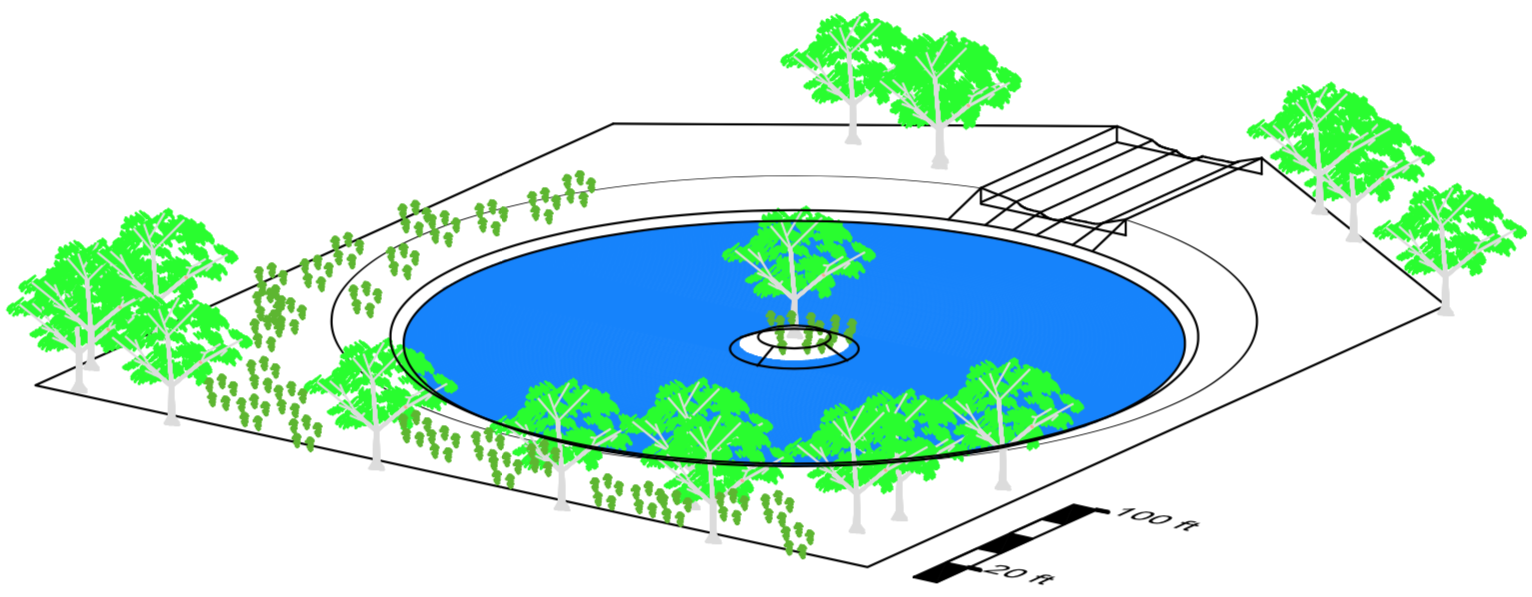
\includegraphics[height=.2\textheight]{F3P.png}
    \caption{Impression of what the pond may look like after landscaping. }
\end{figure}

%%%%%%%%%%%%%%%%%%%%%%%%%%%%%%%%%%%%%%%%%%%%%%%%%%%%%%%%%%%%%%%%%%
%%%%%%%%%%%%%%%%%%%%% 8.0 Required Resources %%%%%%%%%%%%%%%%%%%%%
%%%%%%%%%%%%%%%%%%%%%%%%%%%%%%%%%%%%%%%%%%%%%%%%%%%%%%%%%%%%%%%%%%

\setcounter{figure}{0}
\setcounter{section}{0}
\setcounter{table}{0}
\chapter{Required Resources}


%%%%%%%%%%%%%%%%%%%%%%%%%%%%%%%%%%%%%%%%%%%%%%%%%%%%%%%%%%
%%%%%%%%%%%%%%%%%%%%% 9.0 References %%%%%%%%%%%%%%%%%%%%%
%%%%%%%%%%%%%%%%%%%%%%%%%%%%%%%%%%%%%%%%%%%%%%%%%%%%%%%%%%


\setcounter{figure}{0}
\setcounter{section}{0}
\setcounter{table}{0}
\chapter{References}

%%%%%%%%%%%%%%%%%%%%%%%%%%%%%%%%%%%%%%%%%%%%%%%%%%%%%%%%%%%
%%%%%%%%%%%%%%%%%%%%% 10.0 Appendix A %%%%%%%%%%%%%%%%%%%%%
%%%%%%%%%%%%%%%%%%%%%%%%%%%%%%%%%%%%%%%%%%%%%%%%%%%%%%%%%%%

\setcounter{figure}{0}
\setcounter{section}{0}
\setcounter{table}{0}
\chapter{Appendix A - Resumes}


\renewcommand{\thefigure}{A.\arabic{figure}}
\setcounter{figure}{0}


\begin{flushleft}
\newpage
\bibliography{bib} 
\bibliographystyle{ieeetr} 
\end{flushleft}

\end{document}
